\documentclass[review]{elsarticle}

\usepackage{lineno,hyperref}
\modulolinenumbers[5]

\journal{Journal of \LaTeX\ Templates}

%%%%%%%%%%%%%%%%%%%%%%%
%% Elsevier bibliography styles
%%%%%%%%%%%%%%%%%%%%%%%
%% To change the style, put a % in front of the second line of the current style and
%% remove the % from the second line of the style you would like to use.
%%%%%%%%%%%%%%%%%%%%%%%

%% Numbered
%\bibliographystyle{model1-num-names}

%% Numbered without titles
%\bibliographystyle{model1a-num-names}

%% Harvard
%\bibliographystyle{model2-names.bst}\biboptions{authoryear}

%% Vancouver numbered
%\usepackage{numcompress}\bibliographystyle{model3-num-names}

%% Vancouver name/year
%\usepackage{numcompress}\bibliographystyle{model4-names}\biboptions{authoryear}

%% APA style
%\bibliographystyle{model5-names}\biboptions{authoryear}

%% AMA style
%\usepackage{numcompress}\bibliographystyle{model6-num-names}

%% `Elsevier LaTeX' style
\bibliographystyle{elsarticle-num}
%%%%%%%%%%%%%%%%%%%%%%%

\begin{document}

\begin{frontmatter}

\title{Brazilian Steam Players Analysis}


%% Group authors per affiliation:
\author{Homero Barros}

\author{Lavinia Paganini}


\begin{abstract}
The times when Brazil was out of the world gaming are long gone. Even with bad quality connexions and absurdly high taxes Brazil fellow gamers are getting more and more hardcore everyday. Such a complex country player base has it's own peculiarities and patterns. During the course of this document we will unravel the spicy taste of Brazilian gamers and try to offer a prediction method to what genre of games can find successfulness in this chaotic gaming environment.  
\end{abstract}

\begin{keyword}
Prediction, environment 
\end{keyword}

\end{frontmatter}

\linenumbers

\section{Introduction}

On September 2003 the world most famous gaming platform, Steam, came to life. Breaking the old physical discs gaming paradigm, Steam quickly arise as the gamers favorite choice. With cheap prices, practicality, innovative game sharing and friend connexion Steam conquered a legion of fans in Brazil. Because of Steam's influence in Brazilian market we decided to track down the preferences of the Brazilian player base aiming to predict the most fruitful game genres. On the following section we shall enlighten what approaches where used to find such result. 


\section{Project Steps}
\subsection{Initial Data Mining}
Using the steam data mining API we gathered a large number of Brazilian players profiles. By using each profile we could reach even more profiles by accessing their friend list. Using this functionality we could build data frames like the one in figure 1.


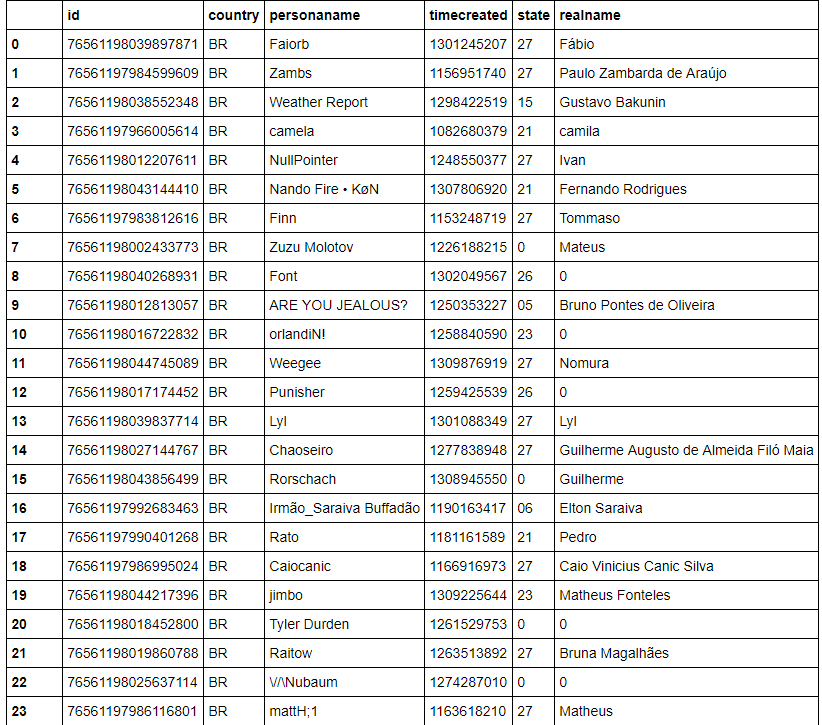
\includegraphics[width=\textwidth]{dataframe.png}

{Figure 1 : Dataframe example}

\subsection{Game information gathering}
After obtaining the player information we started to correlate the player to it's games. We data mined the total playtime and the playtime within two weeks of each game the owner possessed. We also collected game id's so we could mine it's own data. After this we ended with data frames that represented the playtime of all games the player base had like the one represented below.

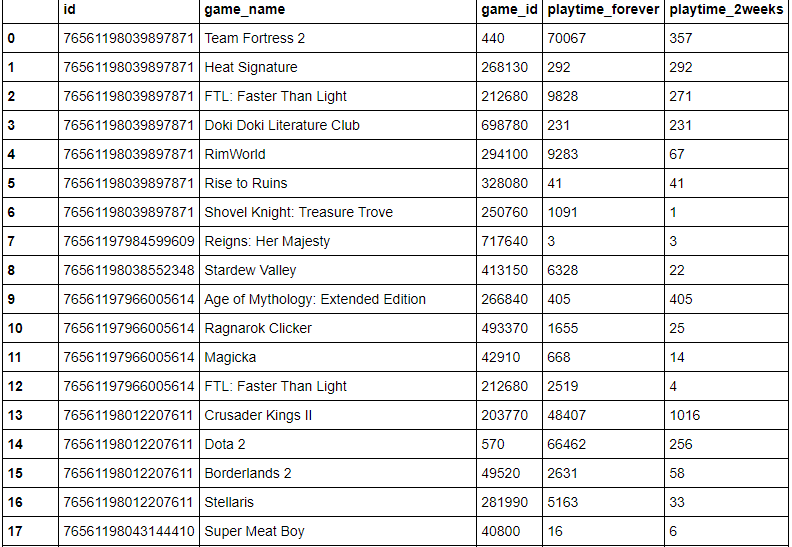
\includegraphics[width=\textwidth]{dataframe2.png}

{Figure 2 : Games Dataframe example}

\subsection*{Game genre mining}
Provided of the games that every player had we then data mined what genre of games each player played. The player id was associated with it's state so we could then map what types of games were played in each state of Brazil and ended up with a data framed that contained each genre correlated with a state.

\subsection{Data training}
Provided of the correlation of genre and states we then created a boolean matrix and used it to train our data. Genres that were present on the game were given the value one where absent genres would be given the value zero. To train our data we used a supervised training algorithm, the random forest. Having divided the dataset in two separate sets, training and test, we could infer the accuracy of our prediction. Given an input genre we return as an output the possible playtime of the genre given the playtime that the player base had based on that genre of game. 

\section{Conclusion}
With this project we could verify how each Brazil region behaves and we we were able to achieve a more generic information about each state genre preference. We worked with a relatively large amount of data, and given our data training we achieved an accuracy of 0.38 on playtime prediction by genre. We could yet confirm old assumptions about Brazil inequality of Internet. This project was a perfect initiation on the data science area. We could experience the very challenges of the data mining and data training and we had yet a little taste on how complex a player base can be.

\end{document}